\section{Evaluation}\label{sec:eval}

Our evaluation answers eight questions.
\textbf{Q1 (\S\ref{subsec:eval_execution_time}):} How much does \sysname{} reduce E2E execution time compared with other systems?
\textbf{Q2 (\S\ref{subsec:eval_success_rate}):} How much does \sysname{} increase profiling feedback?
\textbf{Q3 (\S\ref{subsec:eval_resource_utilization}):} Does \sysname{} keep validation/profiling GPUs busy during the generation phase?
\textbf{Q4 (\S\ref{subsec:eval_performance_breakdown}):} Which components contribute to the E2E speedup?
\textbf{Q5 (\S\ref{subsec:eval_kernel_perf}):} Does speculative generation improve final kernel performance rather than trading performance for shorter iterations?
\textbf{Q6 (\S\ref{subsec:eval_token_consumption}):} What additional token overhead does \sysname{} introduce?
\textbf{Q7 (\S\ref{subsec:eval_harder_tasks}):} Does \sysname{} remain effective on harder \texttt{KernelBench} Level~2/3 tasks?
\textbf{Q8 (\S\ref{subsec:eval_termination_analysis}):} How do E2E time and final kernel performance change with different termination criteria?

\begin{table}[t]
    \centering
    \caption{Short names of ten \texttt{KernelBench} Level~2/3 kernel
    optimization tasks in our extended experiments.}
    \vspace{-10pt}
    \label{tab:tasks_level_2_and_3}
    \small
    \setlength{\tabcolsep}{3pt}
    \renewcommand{\arraystretch}{0.9}
    \begin{tabular}{@{}llll@{}}
    \toprule
    \textbf{Abbr.} & \textbf{Task} & \textbf{Abbr.} & \textbf{Task} \\
    \midrule
    T11 & Gemm $\times$ LeakyReLU   & T16 & Conv2d-BN-Scale \\
    T12 & Gemm Div-Sum-Scale         & T17 & Gemm-Add-ReLU \\
    T13 & Gemm-Scale-BN              & T18 & Matmul-GELU-Softmax \\
    T14 & Conv2d-Act-BN              & T19 & MLP (Level 3) \\
    T15 & Matmul-Sigmoid-Sum         & T20 & ReLU Self-Attn (Level 3) \\
    \bottomrule
    \end{tabular}
    \vspace{-15pt}
\end{table}
\subsection{Experimental Setup}\label{subsec:eval_setup}
\noindent\textbf{Testbed \& Models.}
Our experiments use up to 18 H200 GPUs in our internal cluster. Each node is interconnected via NVLink and RoCEv2 and hosts an Intel Xeon Platinum 8558 CPU.
We serve GLM-5.1 via vLLM with 8 GPUs, while the remaining GPUs are dedicated to validation and profiling.
DeepSeek-V4-Pro is accessed via its official API with high reasoning effort.
The software stack includes PyTorch 2.10, CUDA 12.9, NCU 2025.1.0, and Ninja.
For both models, temperature is set to 0.1 to maintain sharp code-generation formats, and speculative forks disable the reasoning traces.


\begin{figure*}[t]
    \centering
    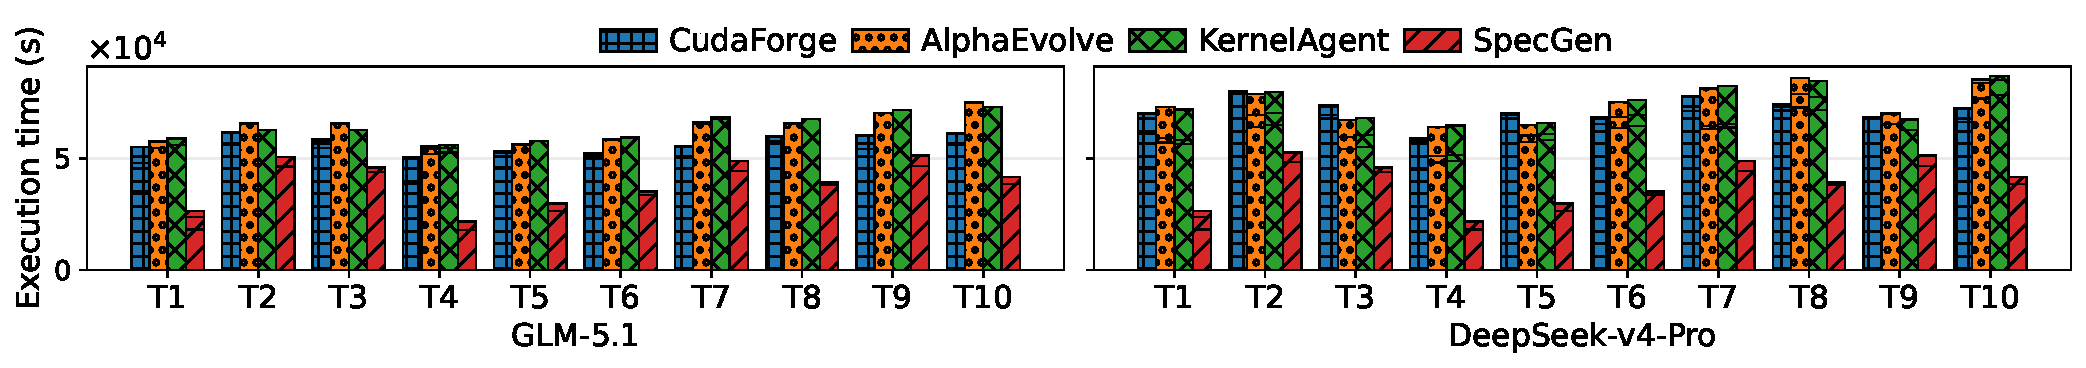
\includegraphics[width=\linewidth]{figs/task_total_time_baseline_vs_spec95_histavg_openevolve_kernelagent_dual_GLM_5_1_vs_dsv4_pro.pdf}
    \vspace{-27pt}
    \caption{End-to-end execution time of 100 iterations per task on GLM-5.1 and DeepSeek-V4-Pro.}
    \vspace{-15pt}
    \label{fig:e2e_execution_time}
\end{figure*}

\begin{figure*}[t]
    \centering
    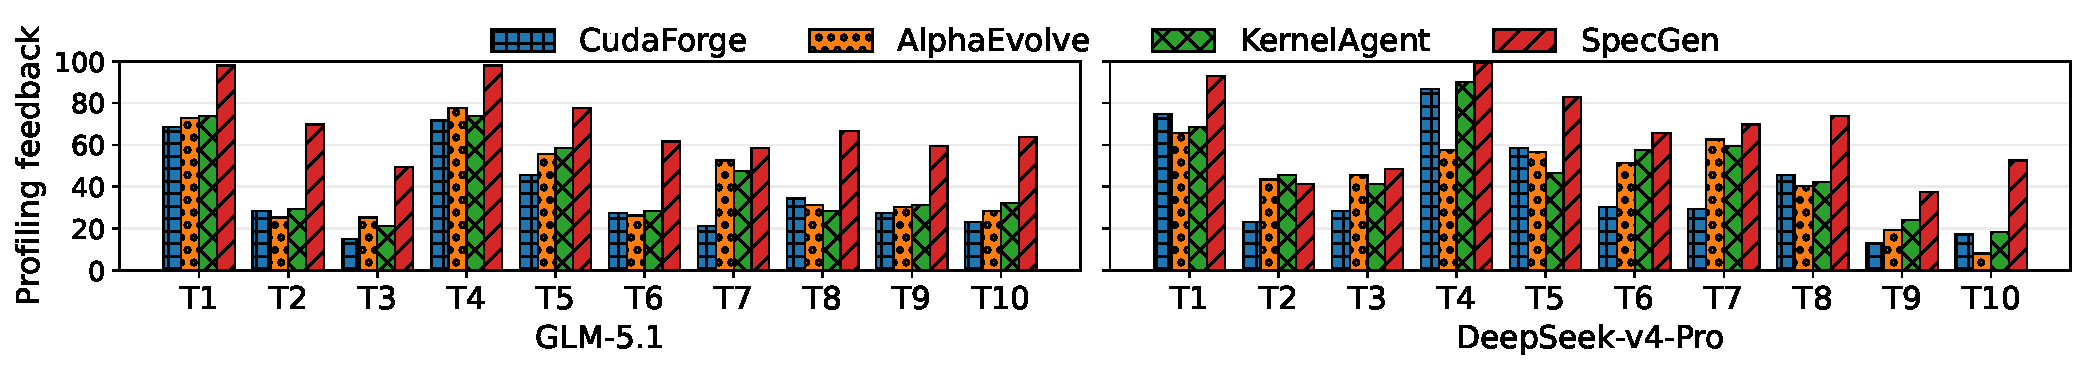
\includegraphics[width=\linewidth]{figs/task_profiling_feedback_rate_speckergen_openevolve_kernelagent_dual_GLM_5_1_vs_dsv4_pro.pdf}
    \vspace{-26pt}
    \caption{Profiling feedback of 100 iterations per task on GLM-5.1 and DeepSeek-V4-Pro.}
    \vspace{-15pt}
    \label{fig:profiling_feedback_rate_lift}
\end{figure*}

\noindent\textbf{Workloads \& Metrics.}
We evaluate the ten KernelBench Level~1 tasks (Table~\ref{tab:tasks}) and ten Level~2/3 tasks (Table~\ref{tab:tasks_level_2_and_3}) with a budget of 100 iterations per task.
To filter device noise, each kernel's speedup over the PyTorch reference is averaged across 40 timed runs (following 10 warmups).
All cross-task aggregated results report the geometric mean.

\noindent\textbf{Baseline.}
We compare \sysname{} against three representative agentic kernel 
optimization systems.
\textbf{(1) CudaForge}~\cite{cudaforge} is a training-free multi-agent 
framework that employs a Coder-Judge workflow to iteratively generate 
and optimize CUDA kernels, guided by hardware feedback from NCU metrics.
\textbf{(2) AlphaEvolve}~\cite{AlphaEvolve} is a coding 
agent from Google DeepMind that pairs reasoning LLMs with automated 
evaluators, using an evolutionary algorithm to iteratively discover 
and refine kernel performance.
\textbf{(3) KernelAgent}~\cite{kernelagent2025} is an autonomous 
kernel generation system from Meta. It 
combines problem analysis, parallel LLM-assisted kernel 
generation with numerical verification, and a hardware-guided 
iterative optimization loop to tune kernel performance.

\subsection{End-to-End Execution Time}\label{subsec:eval_execution_time}

\sysname{} consistently reduces E2E execution time and provides final kernels with 
higher speedups than the three agentic kernel optimization baselines (see Figure~\ref{fig:token_kernel_speedups_GLM_5_1}).

\noindent\textbf{Overall time speedup.}
Figure~\ref{fig:e2e_execution_time} shows that across ten \texttt{KernelBench} tasks, \sysname{} 
achieves a geomean time speedup of 1.50$\times$ over CudaForge on GLM-5.1 and 1.88$\times$ on
DeepSeek-V4-Pro.
Against AlphaEvolve, the geomean speedups are 1.68$\times$ on GLM-5.1 and
1.96$\times$ on DeepSeek-V4-Pro.
Against KernelAgent, the geomean speedups are 1.69$\times$ and 1.96$\times$,
respectively.
Across both models, \sysname{} improves end-to-end time by 1.68$\times$ over
CudaForge, 1.81$\times$ over AlphaEvolve, and 1.82$\times$ over KernelAgent in
geomean.

\noindent\textbf{Long generation latency prolongs iteration time.}
CudaForge follows an iterative Coder-Judge workflow that waits for each
reasoning generation to finish before validation and profiling can provide
hardware feedback.
AlphaEvolve uses an evolutionary loop with automated evaluators, but each
program variant still becomes actionable only after the LLM finishes producing
it.
KernelAgent adds static analysis, parallel kernel generation, strict numerical
verification, and hardware-guided optimization, but its validation and profiling
pipeline also depends on completed candidate kernels.
As a result, these systems mainly improve the search policy after candidates
exist, while validation/profiling resources remain idle during long reasoning
generations.

\noindent\textbf{Early termination reduces generation latency.}
\sysname{} changes the timing of candidate availability.
SpecController forks non-reasoning generations from reasoning prefixes while the
reasoning generation continues as a fallback.
When a speculative kernel satisfies the termination criterion, \sysname{}
terminates the reasoning generation early and advances the iteration.
This mechanism directly reduces the longest phase of each iteration.

% \begin{figure*}[t]
%     \centering
%     \includegraphics[width=\linewidth]{figs/task_speedup_100iter_norm_sg_dual_GLM_5_1_vs_dsv4_pro.pdf}
%     \vspace{-25pt}
%     \caption{Per-task final speedup over the \texttt{KernelBench} reference. Speedup is normalized to \sysname{}.}
%     \vspace{-10pt}
%     \label{fig:final_speedups}
% \end{figure*}

\subsection{Profiling Feedback}\label{subsec:eval_success_rate}

\sysname{} substantially raises profiling feedback through two effects:
it produces more candidate kernels per iteration, and it conditions
non-reasoning generations on reasoning prefixes to improve kernel performance.

\noindent\textbf{Overall feedback increment.}
As shown in Figure~\ref{fig:profiling_feedback_rate_lift}, on GLM-5.1, \sysname{} raises the average profiling feedback to 70.3,
compared with 36.3 for CudaForge, 42.5 for AlphaEvolve, and 42.4 for
KernelAgent.
This corresponds to geomean lifts of 2.13$\times$, 1.78$\times$, and
1.77$\times$, respectively.
On DeepSeek-V4-Pro, \sysname{} reaches 66.4, compared with 40.7 for
CudaForge, 45.1 for AlphaEvolve, and 49.4 for KernelAgent.
The corresponding geomean lifts are 1.84$\times$, 1.61$\times$, and
1.40$\times$.
Across both models, \sysname{} increases profiling feedback by
1.98$\times$ over CudaForge, 1.69$\times$ over AlphaEvolve, and 1.58$\times$
over KernelAgent in geomean.

\noindent\textbf{More candidates per iteration.}
CudaForge, AlphaEvolve, and KernelAgent differ in search policy, but all three
must wait for completed candidate kernels before validation and profiling can
return feedback.
CudaForge uses hardware-feedback-guided agent iteration, AlphaEvolve uses
evolutionary program refinement, and KernelAgent combines analysis, parallel
generation, verification, and hardware-guided tuning.
These mechanisms improve how candidates are selected and refined after they
exist, but they do not expose validation/profiling to useful kernels during the
reasoning generation.
\sysname{} instead forks speculative non-reasoning generations within the same
iteration, so validation sees more candidate kernels under the same iteration
budget.
This increases the chance that at least one candidate passes validation and
reaches profiling.

\noindent\textbf{Faster speculative candidates.}
\sysname{} conditions each speculative generation on the reasoning prefix, which
passes kernel-design decisions from the reasoning trace into the
non-reasoning prompt.
This prefix conditioning improves the performance of speculative kernels and raises
the probability that each additional candidate reaches profiling.
The combination of more and faster candidates improves profiling
feedback across baselines and models.

\subsection{Validation/Profiling Resource Utilization}\label{subsec:eval_resource_utilization}

% \begin{table}[t]
% \centering
% \caption{Validation/profiling resource utilization. Utilization is the percentage of E2E execution time during which validation/profiling GPUs are busy. ES refers to ElasticScheduler.}
% \vspace{-10pt}
% \label{tab:resource_utilization}
% \begin{tabular}{lcc}
%     \toprule
%     Systems & GLM-5.1 & DeepSeek-V4-Pro \\
%     \midrule
%     CudaForge                        &  4.7\% & 11.3\% \\
%     AlphaEvolve                      &  5.0\% & 17.6\% \\
%     KernelAgent                      &  4.2\% & 14.2\% \\
%     \sysname{} w/o ES  & 56.2\% & 74.7\% \\
%     \sysname{}                       & 88.2\% & 96.1\% \\
%     \bottomrule
% \end{tabular}
% \vspace{-10pt}
% \end{table}

\begin{table}[t]
\centering
\caption{Validation/profiling resource utilization. Utilization is the percentage of E2E time during which resources are busy. ES refers to ElasticScheduler. CF: CudaForge, AE: AlphaEvolve, KA: KernelAgent, \textbf{SKG: \sysname{}}.}
\vspace{-10pt}
\label{tab:resource_utilization}
\setlength{\tabcolsep}{4.5pt}
\renewcommand{\arraystretch}{0.9}
\begin{tabular}{lccccc}
    \toprule
    Models & CF & AE & KA & SKG w/o ES & SKG \\
    \midrule
    GLM   & 4.7\% & 5.0\% & 4.2\% & 56.2\% & \textbf{88.2\%} \\
    DSv4  & 11.3\% & 17.6\% & 14.2\% & 74.7\% & \textbf{96.1\%} \\
    \bottomrule
\end{tabular}
\vspace{-15pt}
\end{table}

\begin{figure}[t]
    \centering
    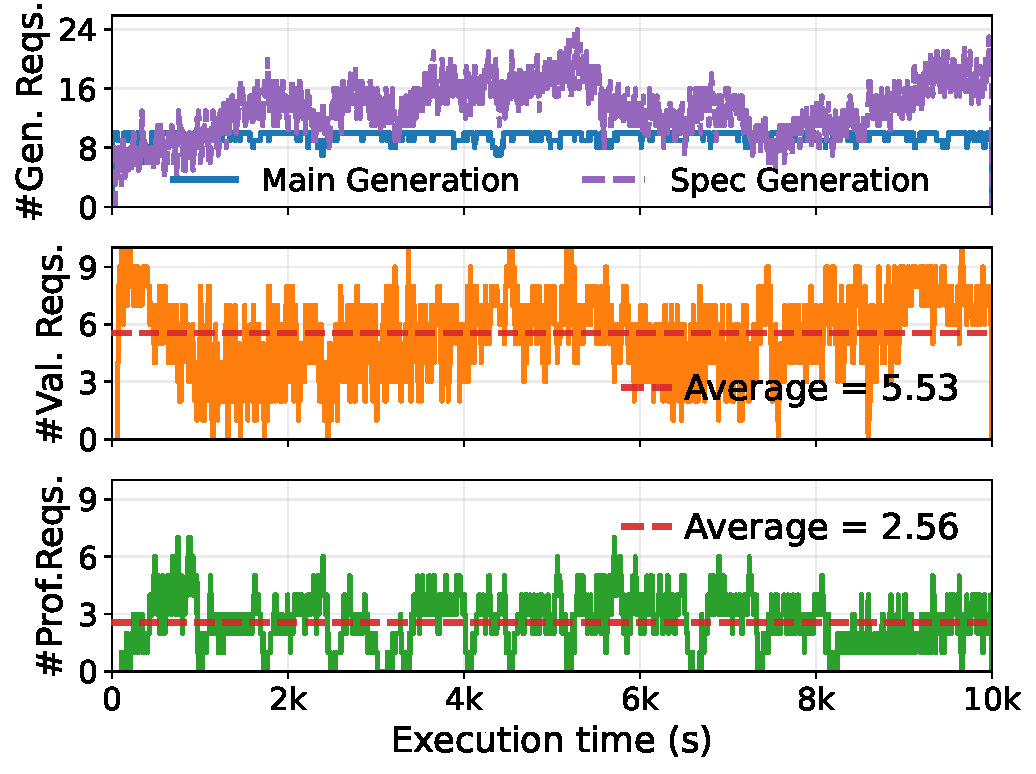
\includegraphics[width=\linewidth]{figs/phase_timeline_combined_GLM_5_1.pdf}
    \vspace{-25pt}
    \caption{In-flight request counts per phase over the first 10{,}000 seconds of \sysname{} on GLM-5.1.}
    \vspace{-15pt}
    \label{fig:phase_timeline_GLM_5_1}
\end{figure}


\begin{figure*}[t]
    \centering
    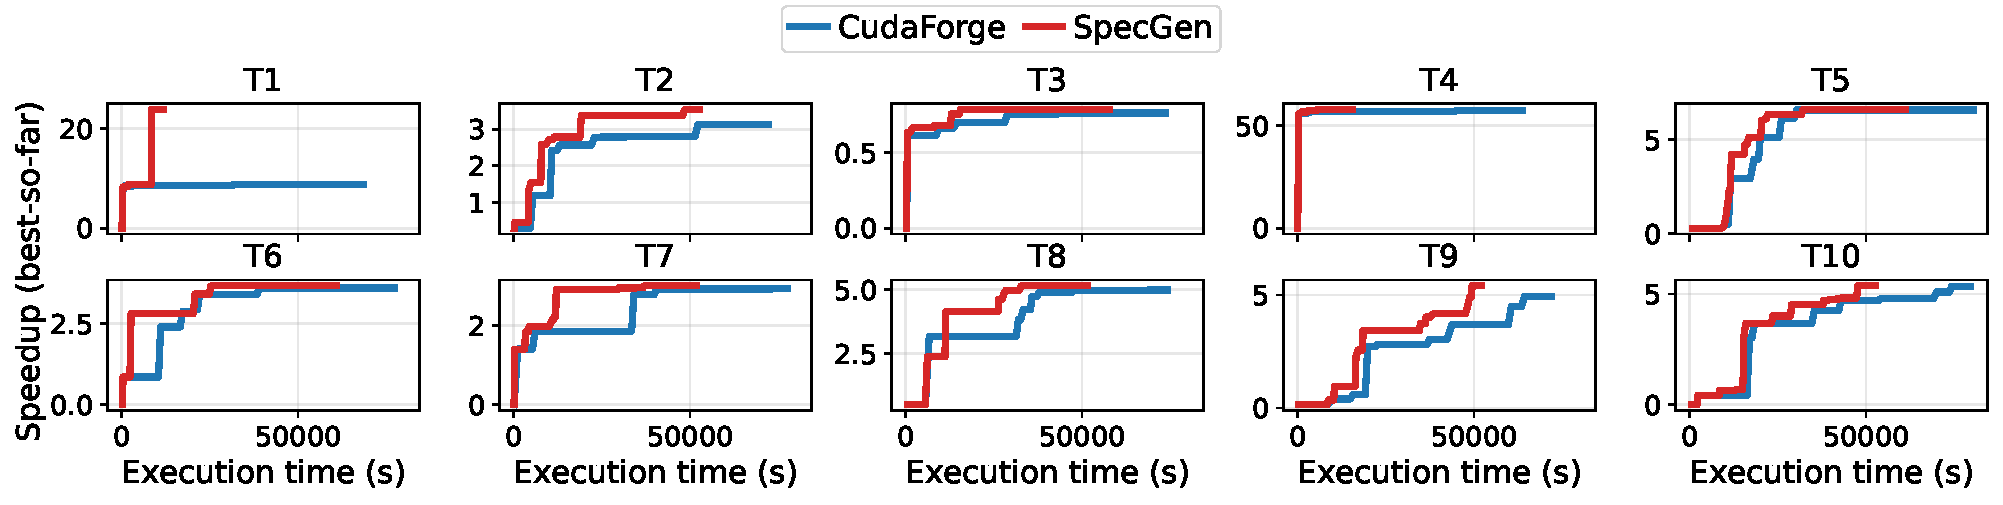
\includegraphics[width=\linewidth]{figs/token_speedup_concat_three_histavg_time_grid_2x5_GLM_5_1.pdf}
    \vspace{-25pt}
    \caption{Detailed time-to-speedup over the \texttt{KernelBench} reference across 100 iterations per task on GLM-5.1.}
    \label{fig:token_kernel_speedups_GLM_5_1}
    \vspace{-12pt}
\end{figure*}

\sysname{} substantially improves validation/profiling resource utilization with SpecController and ElasticScheduler.
\noindent\textbf{Overall utilization lift.}
Table~\ref{tab:resource_utilization} shows that the three baseline systems leave
most validation/profiling capacity idle.
On GLM-5.1, their utilization stays between 4.2\% and 5.0\%; on
DeepSeek-V4-Pro, it stays between 11.3\% and 17.6\%.
\sysname{} without ElasticScheduler already raises utilization to 56.2\% on
GLM-5.1 and 74.7\% on DeepSeek-V4-Pro via emitting additional speculative
candidate kernels.
With ElasticScheduler, utilization further rises to 88.2\% and 96.1\%, showing
that SpecController and ElasticScheduler keep the GPU pool busy under bursty arrivals.

\noindent\textbf{Sporadic validation/profiling requests.}
Since long reasoning generations dominate iteration time, validation/profiling
GPUs wait for completed kernels for most of the run.
The feedback bottleneck is amplified because many generated kernels fail
validation and never reach profiling.
Thus, even methods with stronger search logic or parallel candidate generation
can leave the validation/profiling GPU pool idle.

\noindent\textbf{More requests and bursty handling.}
SpecController increases the number of validation/profiling requests by forking
speculative generations during the reasoning generation.
This alone explains the large jump from baseline utilization to \sysname{}
without ElasticScheduler.
However, speculative requests arrive in bursts, which can leave some GPUs busy
while others are idle under a static split.
ElasticScheduler reallocates validation/profiling capacity based on queue
pressure and adjusts the number of speculative forks when validation/profiling GPUs
become idle or busy.
Figure~\ref{fig:phase_timeline_GLM_5_1} illustrates this behavior over the first
10{,}000 seconds, where validation and profiling remain active instead of waiting
for completed reasoning generations.
The result is near-saturated validation/profiling GPU utilization.


\subsection{Performance Breakdown}\label{subsec:eval_performance_breakdown}

\begin{table}[t]
    \centering
    \caption{Incremental performance breakdown of \sysname{} on GLM-5.1 across ten \texttt{KernelBench} tasks. Speedup is geomean end-to-end time speedup over CudaForge.}
    \vspace{-10pt}
    \label{tab:ablation_study}
    \renewcommand{\arraystretch}{0.9}
    \begin{tabular}{lcc}
        \toprule
        Configuration & Speedup & $\Delta$ \\
        \midrule
        Baseline & 1.00$\times$ & 0.00 \\
        + Speculative Generation & 1.46$\times$ & 0.46$\uparrow$ \\
        + Resource Reallocation & 1.61$\times$ & 0.15$\uparrow$ \\
        + Priority Queue & 1.69$\times$ & 0.08$\uparrow$ \\
        + Remote Prefix Cache & 1.77$\times$ & 0.09$\uparrow$ \\
        \bottomrule
    \end{tabular}
    \vspace{-15pt}
\end{table}
Table~\ref{tab:ablation_study} breaks down where \sysname{}'s end-to-end
speedup comes from.
The first step, speculative generation, accounts for most of the gain by raising
geomean speedup from 1.00$\times$ to 1.46$\times$.
Speculative generation shortens the critical path directly. A speculative
kernel can satisfy the termination criterion before the reasoning generation
finishes, so the iteration no longer has to wait for the reasoning generation.

The remaining components make those speculative kernels useful sooner.
Resource reallocation raises speedup to 1.61$\times$ by moving GPUs toward the
busier validation or profiling phase, which reduces idle time under bursty
speculative arrivals.
Priority queues further raise speedup to 1.69$\times$ by validating later-prefix
candidates first and returning profiling feedback in FIFO order.
Together, these scheduling mechanisms reduce validation/profiling waiting time,
which lets SpecController receive results earlier and trigger early termination
sooner.
Remote prefix caching completes the system by raising speedup to 1.77$\times$.
It lets speculative generations reuse the cached reasoning prefix instead of
recomputing shared prompt state, so the system can add speculative branches with
only modest extra generation cost.


\subsection{Kernel Performance}\label{subsec:eval_kernel_perf}


\begin{table}[t]
    \centering
    \small
    \setlength{\tabcolsep}{2pt}
    \caption{Best kernel speedup over the \texttt{KernelBench} reference. The first block reports GLM and the second block reports DeepSeek. \ding{55}: no available kernels. CF: CudaForge, AE: AlphaEvolve, KA: KernelAgent, \textbf{SKG: \sysname{}}.}
    \vspace{-10pt}
    \label{tab:final_kernel_perf}
    \begin{tabular}{lcccccccccc}
        \toprule
        System & T1 & T2 & T3 & T4 & T5 & T6 & T7 & T8 & T9 & T10 \\
        \midrule
        CF   & 8.81 & 3.12 & 0.76 & 57.23 & 6.56 & 3.60 & 2.92 & 4.97 & 4.94 & 5.34 \\
        AE & 12.83 & 1.61 & \ding{55} & 47.43 & 2.45 & 0.81 & 0.69 & 4.15 & 3.98 & 2.36 \\
        KA & 21.23 & 2.21 & \ding{55} & 56.98 & 4.97 & 2.57 & 2.60 & 4.31 & 5.11 & 4.67 \\
        \textbf{SKG}  & \textbf{23.86} & \textbf{3.54} & \textbf{0.79} & \textbf{57.72} & \textbf{6.60} & \textbf{3.66} & \textbf{2.99} & \textbf{5.13} & \textbf{5.41} & \textbf{5.37} \\
        \midrule
        CF   & 8.64 & 0.88 & 0.86 & 60.87 & 4.76 & 3.61 & 2.30 & 3.72 & 0.53 & 0.46 \\
        AE & 7.98 & 0.53 & 0.61 & 59.47 & 1.00 & 3.36 & 1.29 & 3.11 & 0.82 & 0.71 \\
        KA & 6.17 & 0.23 & 0.05 & 61.15 & 4.98 & 4.32 & 2.29 & 3.50 & 1.02 & 0.69 \\
        \textbf{SKG}  & \textbf{8.76} & \textbf{1.69} & \textbf{0.90} & \textbf{61.54} & \textbf{5.38} & \textbf{5.94} & \textbf{3.00} & \textbf{3.87} & \textbf{1.19} & \textbf{0.73} \\
        \bottomrule
    \end{tabular}
    \vspace{-15pt}
\end{table}

\sysname{} improves kernel performance and finds faster kernels within
fixed time budget with early termination.

\noindent\textbf{Overall kernel performance.}
Table~\ref{tab:final_kernel_perf} shows the best kernel speedup over
the \texttt{KernelBench} reference after 100 iterations.
On both GLM-5.1 and DeepSeek-V4-Pro, \sysname{} obtains the best final kernel on
all ten tasks.
Its geomean speedup over the reference reaches 5.78$\times$ on GLM-5.1 and
3.49$\times$ on DeepSeek-V4-Pro.
Across both models, this corresponds to geomean lifts of 1.24$\times$ over
CudaForge, 1.91$\times$ over AlphaEvolve, and 1.52$\times$ over KernelAgent.

\noindent\textbf{Faster kernel within fixed time budget.}
In this experiment, \sysname{} stops the reasoning generation only after a
speculative kernel exceeds the average speedup of previously profiled kernels.
Figure~\ref{fig:token_kernel_speedups_GLM_5_1} shows that with early termination,
\sysname{} finds faster kernels than CudaForge within the fixed time budget.
Across all tasks, the best-so-far speedup trajectory of \sysname{} reaches or exceeds
the CudaForge trajectory by the end of the execution.
The final results in Table~\ref{tab:final_kernel_perf} further confirm that
speculative generation and early termination improve kernel performance while reducing
the end-to-end execution time.

\subsection{Overhead of \sysname{}}\label{subsec:eval_token_consumption}

\sysname{} introduces modest token overhead with prefix caching and early termination.

\begin{table}[t]
    \centering
    \small
    \setlength{\tabcolsep}{2.3pt}
    \caption{Token consumption (millions) of \sysname{} relative to CudaForge across 100 iterations on GLM-5.1. Ratio is \sysname{} tokens divided by CudaForge tokens.}
    \vspace{-10pt}
    \label{tab:token_overhead}
    \begin{tabular}{lcccccccccc}
        \toprule
        & T1 & T2 & T3 & T4 & T5 & T6 & T7 & T8 & T9 & T10 \\
        \midrule
        CudaForge & 1.98 & 2.42 & 2.42 & 2.05 & 2.64 & 2.38 & 2.50 & 2.41 & 2.38 & 2.47 \\
        \sysname{} & 0.89 & 2.71 & 2.51 & 1.06 & 3.13 & 2.72 & 2.51 & 2.55 & 2.44 & 2.62 \\
        Ratio & 0.45 & 1.12 & 1.04 & 0.52 & 1.18 & 1.14 & 1.01 & 1.06 & 1.02 & 1.06 \\
        \bottomrule
    \end{tabular}
    \vspace{-15pt}
\end{table}

\noindent\textbf{Overall token cost.}
Table~\ref{tab:token_overhead} shows that \sysname{}'s total token consumption is
slightly lower than CudaForge despite launching speculative generations.
Across all ten tasks, CudaForge consumes 23.66M tokens, while \sysname{} consumes
23.14M tokens, or 0.98$\times$ of CudaForge.
Most matmul tasks incur modest extra tokens, with ratios between 1.01$\times$
and 1.18$\times$.
However, HingeLoss (T1) and diagonal matmul (T4) terminate early in many
iterations.
Their reasoning generations are therefore cut short, saving most of the
tokens that would otherwise be spent after the useful speculative kernel has
already appeared.
As a result, T1 and T4 consume only 0.45$\times$ and 0.52$\times$ of CudaForge's
tokens, which offsets the modest overhead on harder tasks.

\noindent\textbf{Prefix caching and early termination offset token overhead.}
\sysname{} concatenates the original prompt with the current
reasoning prefix to form the speculative prompt. Therefore, the prefill of speculative generations can reuse the KV cache of the reasoning generation.
Moreover, early termination also saves tokens.
Both effects offset the modest overhead across these ten tasks.

\subsection{Performance on Harder Tasks}\label{subsec:eval_harder_tasks}
\begin{table}[t]
\centering
\caption{Results on T11--T20 (Level~2/3) with DeepSeek. Each task runs 100 iterations. CF: CudaForge, SKG: \textbf{\sysname{}}.}
\vspace{-10pt}
\label{tab:comparison-t11-t20}
\small
\setlength{\tabcolsep}{2.3pt}
\renewcommand{\arraystretch}{0.9}
\begin{tabular}{@{}l cc cc cc cc cc@{}}
    \toprule
    & \multicolumn{2}{c}{E2E (k s)} & \multicolumn{2}{c}{Prof.\ FB} & \multicolumn{2}{c}{Util. (\%)} & \multicolumn{2}{c}{Speedup} & \multicolumn{2}{c}{Tokens (M)} \\
    \cmidrule(lr){2-3}\cmidrule(lr){4-5}\cmidrule(lr){6-7}\cmidrule(lr){8-9}\cmidrule(lr){10-11}
    Task & CF & SKG & CF & SKG & CF & SKG & CF & SKG & CF & SKG \\
    \midrule
    T11 & 37.6 & \textbf{24.5} & 21.2 & \textbf{41.3} & 13.6 & \textbf{94.3} & 0.60 & \textbf{1.25} & 1.20 & 1.27 \\
    T12 & 32.2 & \textbf{21.0} &  1.0 & \textbf{13.2} & 14.9 & \textbf{81.2} & 0.01 & \textbf{0.42} & 0.92 & 1.45 \\
    T13 & 39.3 & \textbf{21.5} & 22.2 & \textbf{63.6} & 14.5 & \textbf{84.8} & 0.63 & \textbf{0.63} & 1.40 & 1.12 \\
    T14 & 34.4 & \textbf{22.6} & 37.4 & \textbf{51.5} & 19.2 & \textbf{91.2} &  1.65 & \textbf{1.68} & 1.01 & 1.22 \\
    T15 & 40.2 & \textbf{18.3} & 29.3 & \textbf{69.7} & 15.2 & \textbf{86.3} &  0.74 & \textbf{0.77} & 1.19 & 1.96 \\
    T16 & 35.8 & \textbf{17.0} & 37.4 & \textbf{73.7} & 19.2 & \textbf{92.4} &  1.06 & \textbf{1.27} & 1.27 & 1.18 \\
    T17 & 38.3 & \textbf{22.6} & 24.2 & \textbf{55.6} & 15.2 & \textbf{88.5} &  0.62 & \textbf{0.74} & 1.14 & 1.55 \\
    T18 & 32.7 & \textbf{27.7} &  7.1 & \textbf{31.3} &  8.5 & \textbf{81.1} &  0.35 & \textbf{55.79} & 1.18 & 1.10 \\
    T19 & 61.5 & \textbf{49.0} & 41.9 & \textbf{69.2} & 22.3 & \textbf{93.2} &  0.64 & \textbf{1.05}  & 2.94 & 3.17 \\
    T20 & 55.1 & \textbf{47.2} & 39.4 & \textbf{77.1} & 14.0 & \textbf{89.2} &  1.10 & \textbf{1.39}  & 2.61 & 2.92 \\
    \bottomrule
\end{tabular}
\vspace{-15pt}
\end{table}

\sysname{} remains effective on harder \texttt{KernelBench} Level~2/3 tasks,
improving runtime, feedback density, validation and profiling resource utilization, and
final kernel speedup over the reference with modest token overhead.
Table~\ref{tab:comparison-t11-t20} compares \sysname{} with CudaForge on ten
harder tasks with DeepSeek.
On average, \sysname{} reduces E2E time by 1.57$\times$ and raises profiling
feedback from 26.1 to 54.6.
It also increases resource utilization from 15.7\% to 88.2\%.
Moreover, \sysname{} finds kernels at least as fast as CudaForge on all ten tasks and a
strictly faster kernel on nine of them, improving geomean kernel speedup over
the reference from 0.49$\times$ to 1.42$\times$.
The additional token cost remains moderate, with a 14.0\%
increase in total token consumption.

\subsection{Termination Criterion Analysis}\label{subsec:eval_termination_analysis}

\sysname{} improves kernel performance within a fixed token budget and
exposes a tunable trade-off between E2E time and kernel performance.


\noindent\textbf{More feedback per token yields faster kernels.}
Table~\ref{tab:termination_analysis} compares \sysname{} against CudaForge under
matched token budgets.
Simply doubling CudaForge's token budget barely improves performance, raising the
final speedup from 5.05$\times$ to 5.15$\times$ on GLM and from 2.61$\times$
to 2.74$\times$ on DeepSeek.
\sysname{} with the historical-average criterion reaches 5.78$\times$ and
3.18$\times$ while consuming only 130.2\% of CudaForge's tokens, fewer than
CudaForge$^+$.
The reason is that speculative generations are non-reasoning and reuse the
cached reasoning prefix, so each candidate costs few tokens.
Under the same budget, \sysname{} therefore produces far more profiling feedback
(114.9 and 101.1 additional feedback) than extra reasoning generations would.
This added feedback in return guides the LLM toward faster kernels.

\noindent\textbf{The termination threshold tunes the time-performance trade-off.}
Lowering the threshold trades kernel performance for shorter runtime.
First-valid termination stops earliest, giving the shortest E2E time, 
yet still emits many candidate kernels and reaches
5.53$\times$ and 2.95$\times$, already faster than CudaForge.
The historical-average default sits in the middle, preserving most of the latency
benefit while improving performance.
When tokens are abundant, disabling termination finds the fastest kernels at the cost of more tokens.
Across every criterion, \sysname{} produces faster kernels than CudaForge under a
comparable or smaller token budget.

\begin{table}[t]
    \centering
    \small
    \setlength{\tabcolsep}{3pt}
    \caption{Comparison of CudaForge and \sysname{} with different termination criteria across T1--T10. The first block reports results with GLM and the second reports DeepSeek. CudaForge$^+$: Doubled token budget for CudaForge.}
    \vspace{-10pt}
    \label{tab:termination_analysis}
    \renewcommand{\arraystretch}{0.9}
    \begin{tabular}{lccccc}
        \toprule
        \makecell[l]{Method} & \makecell[c]{\#Additional\\feedback} & \makecell[c]{Kernel\\Speedup} & \makecell[c]{Token\\Ratio} & \makecell[c]{\#Term.} & \makecell[c]{E2E\\time (s)} \\
        \midrule
        CudaForge & 0 & 5.05$\times$ & 100\% & 0 & 73.9k \\
        CudaForge$^+$  & 35.2 & 5.15$\times$ & 208.6\% & 0 & 75.2k \\
        First valid  & 70.0 & 5.53$\times$ & 114.3\% & 70.3 & 39.8k \\
        \textbf{Hist. avg.}  & 114.9 & 5.78$\times$ & 130.2\% & 63.0 & 43.8k \\
        Hist. best  & 535.9 & 6.06$\times$ & 229.5\% & 9.0 & 70.3k \\
        No term.  & 587.2 & 6.15$\times$ & 240.0\% & 0 & 73.9k \\
        \midrule
        CudaForge  & 0 & 2.61$\times$ & 100\% & 0 & 57.0k \\
        CudaForge$^+$  & 44.3 & 2.74$\times$ & 210.9\% & 0 & 57.7k \\
        First valid  & 64.5 & 2.95$\times$ & 105.1\% & 64.5 & 29.6k \\
        \textbf{Hist. avg.}  & 101.1 & 3.18$\times$ & 130.2\% & 52.8 & 35.9k \\
        Hist. best  & 252.3 & 4.79$\times$ & 208.3\% & 8.1 & 54.6k \\
        No term.  & 269.1 & 5.08$\times$ & 218.1\% & 0 & 57.0k \\
        \bottomrule
    \end{tabular}
    \vspace{-15pt}
\end{table}